\documentclass{article}

\usepackage{amsmath}
\usepackage{setspace}
\usepackage{xcolor}
\usepackage{graphicx}
\usepackage{subcaption}
\graphicspath{{figures/}}

\pagecolor{black}
\color{white}
\title{Appunti per Metallurgia e Materiali non Metallici}
\date{19-02-2023}
\author{Matteo Sanderson}

\begin{document}

    \pagenumbering{gobble}
    \maketitle
    \newpage
    \setstretch{1.25}
    \newpage
    \tableofcontents
    \setcounter{tocdepth}{5}
    \newpage
    \pagenumbering{arabic}
    \section{Appunti iniziati}
        \subsection{Libri consigliati}
            \begin{itemize}
                \item Nicomedi - Metallurgia
                \item Nicomedi - Accai e leghe non ferrose
                \item Askeland - The Science and Engineering of Materials
                \item Campbell - Metallurgy and Engineering Alloys
            \end{itemize}
        I concetti sono importanti non le formule
        \subsection{Link}
            \begin{itemize}
                \item fa-fe.com
                \item fa-fe.it
                \item Password: 1141410931181
            \end{itemize}
        \subsection{Modalita' d'esame}
            Parte A (25\% del voto): Domande a risposta multipla. 2 punti per risposta corretta, 0 per nessuna risposta e -1 per risposta errata. Almeno 16 per passare.
            \newline Parte B (75\% del voto): Scritto a risposta aperta, 2 ore per 4 domande. Almeno 18 per passare.         
    \section{Lezione 1 - Introduzione}
            \subsection{Differenze tra metalli e leghe}
                I metalli, come ferro, alluminio, rame e nickel hanno delle leghe e il nome delle leghe gli e' stato dato o viene derivato dei metalli che creano la lega.
                L'accaio e' la lega piu' importante a cause delle sue proprieta' interessanti e il suo costo che e' relativamente basso.
                \newline    Una legha ferrosa con un contentuo minore di 2,11\% di carbonio e' nota come ferro invece una leghe ferrosa con un contenuto di carbonio maggiore di 2,11\% e' nota come ghisa.
                \newline    Ci sono anche leghe di alluminio e rame. Il rame crea leghe con altri metalli, la sua lega con lo stagno e' nota come il bronzo mentre la sua leghe con lo zinco e nota come l'ottone.
                \newline    Il titanio crea leghe ma sono fuori dello scopo del corso a causa dell'uso sparso a colpa del prezzo elevato del titanio.
            \subsection{Legami}
                \subsubsection{Legame Ionico/Ceramiche}
                    I legami ionici vengono creati a cause delle attrazione elettrostaticha tra anioni di non mettalli e cationi di metalli.
                    I legami ionici creano ceramiche. I materiali ceramici hanno molti usi anche in ambiti industriali tra piastrelle, sali e vetri.
                    Tutti i materiali ceramici sono sono composti da legami ionici.
                    \newline Esempi di materiali ceramici includono:
                    \begin{itemize}
                        \item Al\textsubscript{2}O\textsubscript{3} (Allumina)
                        \item SiO\textsubscript{2} (Silice)
                        \item NaCl 
                    \end{itemize}
                
                \subsubsection{Legame Covalente/Polimeri}
                    I polimeri(organici) sono creati da numeri grandi di monomeri, che catene lunghe di carbonio.
                    I polimeri possono esser visti come degli spaghetti, dove se non ci metti l'olio dopo essere cotti possono avere delle proprieta diverse.
                    \newline \newline I polimeri termoplastici sono polimeri che dopo essere formati possono essere ririscaldati per dargli una nuova forma,
                    questo e' perche i materiali sono solo tenuti insieme da legami idrogeni e altri legami deboli che possono riformarsi se rotti.
                    Invece i polimeri termodurenti sono polimeri che quando gli viene data un forma non puo' essere piu' cambiata, questo
                    e' a cause delle retticolazione (cross-linking), che e' un effetto dove i monomeri creano legami covalenti tramite i gruppi funzionali che
                    non possono esser rotti facilmente percio' i polimeri termodurenti di solito bruciano prima di sciogliersi.

                \subsubsection{Legame Metallico}
                    In un legame metallico tutti gli atomi perdono i loro elettroni di valenza e essi vanno nella nube di elettroni che charatterizza un legame metallico.
                    Gli atomi percio' hanno carica positiva mentre la nube ha carica negativa, questo crea una attrazione elettrostatica che mantiene il materiale insieme.
                    \newline Gli atomi si mettono in una retticola a distanze costanti a cause di forze di attrazione e repulsione che ci sono fra gl'atomi e gl'atomi e gl'atomi e la nube di elettroni.
            
            \subsection{Caratterristiche importanti dei legami}
                \hangindent=0.7cm \textbf{Caratteristica importante delle ceramiche:}
                \newline \hangindent=0.7cm Le caratteristiche degli elementi componenti sono perse nelle ceramiche e il materiali guadagna proprieta' sue.
                \newline \newline \textbf{Caratteristica importante dei polimeri:}
                \newline Anche i monomeri perdono le proprieta' degli elementi che li compongono.
                \newline \newline \textbf{Caratteristiche importanti dei composti metallici:}
                \begin{itemize}
                    \item Elevata energia e forza di legame
                    \item Comportamento isotopo (assenza di prorieta' direzionali [come in ceramiche e polimeri])
                    \item Assenza localizzazione della carica elettrica
                    \item Conduttivita' elettrica e termica $\longrightarrow $ Perche elettroni non sono bloccati e invece sono liberi di muoversi influenzare l'un l'altro.
                    \item Alta lucentezza $\longrightarrow $ I fotoni che colpiscono la superfice colpiscono gli elettroni nella nube e vengono assorbiti e sparati indietro(diagrammi Feynman).
                    \item Alta compattezza e densita'
                \end{itemize}

            \subsection{Caratteristica fondamentale dei metalli}
                Tutte le classi di materiali (ceramiche, polimieri e metalli) possono essere deformati plasticamente,
                pero i metalli sono gli unici che possono essere deformati plasticamente senza rompersi.
                \newline \newline La deformazione plastica e' definita da uno scorrimento degl'atomi in una struttura.
                \newline \newline I metalli sono gli unici che possono deformarsi senza rompersi perche la struttura dei metalli non dipende dalla posizione specifica di cariche,
                come nei legami ionici, percio' quando c'e' uno scorrimento gli elettroni mantengono la struttura mentre gli atomi cambiano solo gli atomi sui hanno effetto la loro repulsione.
                \newline \newline Se lo scorrimento occorresse in un retticolo ionico gli anioni e cationi si incontrerebbero e ci sarebbe un repulsione percio' si romperebbe.
                \newline \newline Invece nei polimeri la ragioni sono diverse. Nei polimeri termoplastici con uno scorrimento i legami ad idrogeno si rompono e gli monomeri si muovono,
                 questo puo essere visto un sacchetto che si stira e poi si rompe. Se si tentasse di deformare i monomeri se stessi i monomeri si deformerebbero elasticamente e con abbastanza
                 forza i legami covalenti del monomero si romperebbero. In un polimero termodurente, la deformazione plastica non occorre perche la struttura e' un retticolo grande e percio'
                 si possono solo rompere i legami covalenti percio' cambiando la struttura effettiva.
                 \newline \newline A causa di queste proprieta la ceramiche e i polimieri possono essere chiamati \textcolor{red}{\textbf{Fragili}}. Fragile significa che non occorre deformazione plastica prima
                 che il materiale si rompa. Invece i metalli sono chiamati \textcolor{red}{\textbf{Duttili}}. Duttile significa che dopo abbastanza deformazione plastica il materiale si rompe. La deformazione
                 plastica e' progressiva prima di rompersi, questo e' importante perche' in casi industriali si possono vedere deformazione dei metalli prima che si rompa, percio' e' piu' sicuro.
    \newpage
    \section{Lezione 2 - Retticoli cristallini dei metalli}
        \begin{figure}[h!]
            \centering
            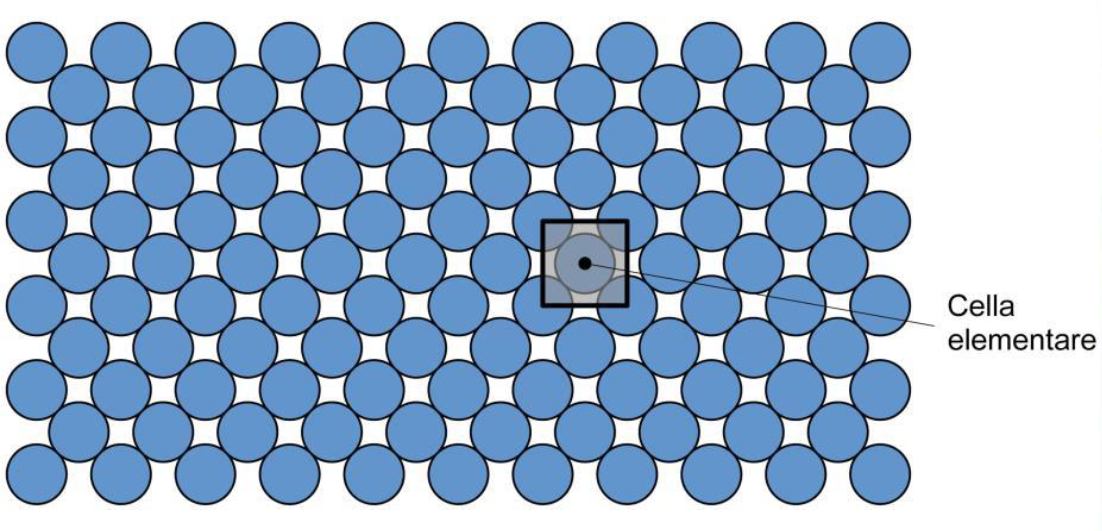
\includegraphics[width=\linewidth]{Retticolo pre 1800.png}
            \caption{Retticolo cristallino dei metalli alla fine dell'1800}
        \end{figure}
        La figura fa vedere l'idea che gli scienziati alla fine del 1800 avevano sulla struttura del retticolo metallico.
        Oltra la ovvia mancanza della nube di elettroni, l'idea e' per la maggior parte la struttura e' giusta.
        \newline \newline La metallurgia spiega le proprieta' macroscopiche con la proprieta' microscopiche del materiale.

        In generale per i materiali metallici piu' deformabile il materiale meno e' rigido e meno e' deformabile piu' e' resistente.

        I materiali mettalici sono disposti in modo regolare noto come un retticolo, questo retticolo e'
         composti da celle elementari che si ripetono e creano il retticolo grande nel metallo.

        \newpage
        \subsection{Tipi di celle elementari}
            \subsubsection{Reticolo cubico a corpo centrato (CCC)}
                \begin{figure}[h!]
                    \centering
                    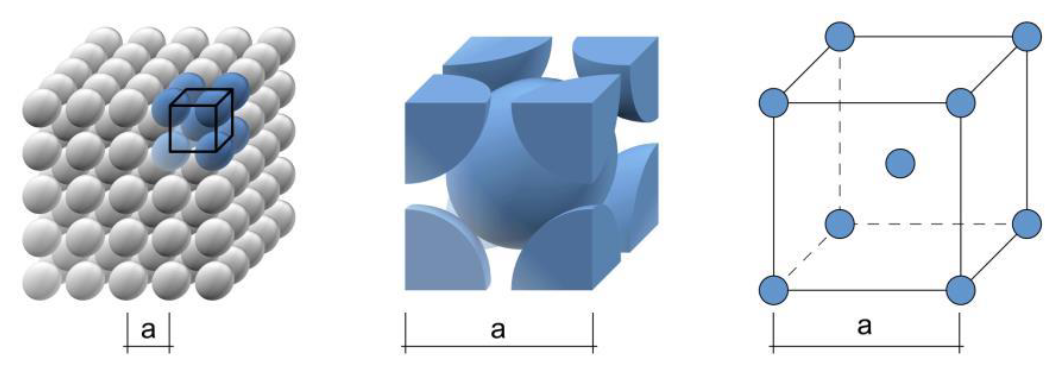
\includegraphics[width=\linewidth]{Reticolo cubico a corpo centrato.png}
                \end{figure}
                In un reticolo cubico a corpo centrato un atomo e' centrato nella cella con altri altri atomi posti ad ogni vertice che comprende l'atomo centrale.
                Gli atomi si toccano lungo la diagonale del cubo.
                \newline \newline Questa strutture per le celle elementari e' usata dal cromio(Cr), vanadio(V), tungsteno(W), molibdeno(Mo), litio(Li), sodio(Na) e calcio(Ca), e' anche
                la struttura del ferro(Fe) quando $T<912^o C$ e quando $1396^o C<T<1538^o C$.
                \newline \newline Il ferro e' un materiale allotropico, che significa che subisce una trasformazione che cambia la forma delle sue celle elementari.
                \newline \newline Il reticolo CCC a due atomi propri che lo compongono.
                \begin{figure}[h!]
                    \centering
                    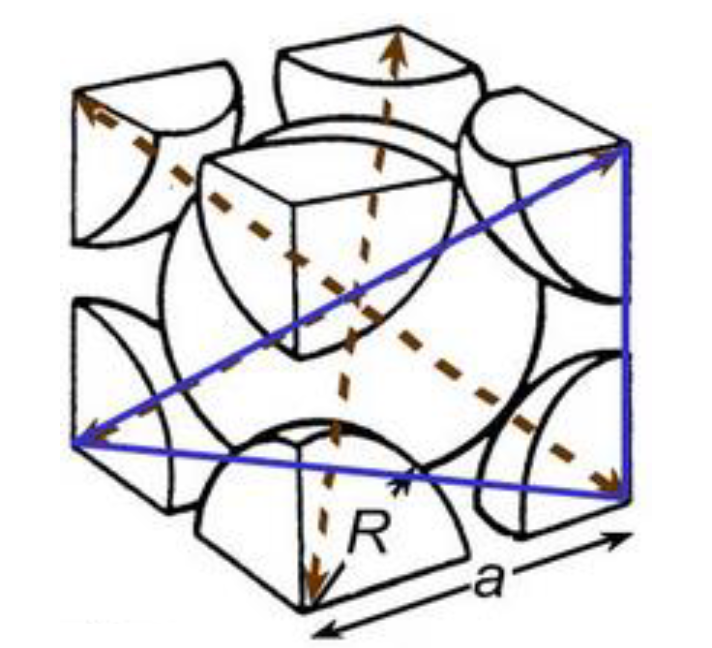
\includegraphics[width=0.5\linewidth]{CCC calcolo}
                \end{figure}
                \begin{gather}
                    (4R)^2 = a^2 + (a \sqrt{2})^2 \\
                    a = \frac{4R}{\sqrt{3}} \label{CCC_reference} \\
                    a^3 = 12,32 R^3
                \end{gather}

            \subsubsection{Fattori di compattazione atomica (APF - Atomic Packing Factor) per il reticolo CCC}
                \paragraph{Definizione di APF} L'APF e' usato per determinare la densita di una cella elementare o potrebbe esser visto come la percentuale del volume in una cella e' occupata da atomi. 
                \begin{equation}
                    APF = \frac{\text{Volume degli atomi nella cella}}{\text{Volume nella cella}}
                \end{equation}
                \begin{gather}
                    V_\text{atomi} = 2 * \frac{4}{3} \pi R^3 \cong 8,37 R^3 \\
                    V_\text{cella} \cong 12,32 R^3 \\
                    APF_\text{CCC} = \frac{V_\text{atomi}}{V_\text{cella}} = \frac{8,37 R^3}{12,32 R^3} \cong 0,68
                \end{gather}

                $\Longrightarrow$ Il volume del reticolo CCC e' occupato il 68\% da atomi.
            
            \subsubsection{Reticolo cubico a facce centrate (CFC)}
                \begin{figure}[h!]
                    \centering
                    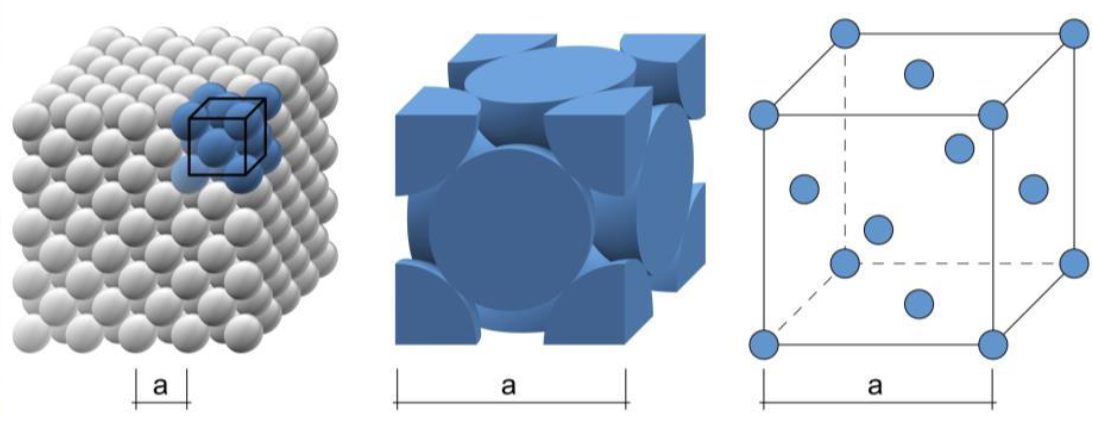
\includegraphics[width=\linewidth]{Reticolo CFC}
                \end{figure}
                Il reticolo CFC e' una struttura piu' complessa del reticolo CCC, questo e' perche il reticolo CFC ha le facce che puntano verso il centro non ha un atomo centrale.
                Questo significa che ci sono 4 atomi propri nel reticolo CFC invece dei 2 del reticolo CCC, e causa il volume del reticolo CFC ad esser piu' grande del reticolo CCC perche 
                la tangenza degli atomi occorrere sulla diagonale delle facce della cella in confronto con la diagonale del cubo intero come nei reticolo CCC.
                \newline \newline Il reticolo CFC e' il reticolo usato dal rame(Cu), argento (Ag), oro (Au), alluminio (Al), nickel(Ni), piombo (Pb), platino(Pt) e 
                il ferro quando $912^o C<T<1396^o C$.
                \newline \newline Tutti i metalli elencati sono noti per la loro deformabilita', quindi si puo' capire il reticolo e' la cause della deformabilita'.
                \newline \newline Il ferro quando entra questa forma diventa piu' maleabile/deformabile, questo spiega perche' i fabbri ferrai riscaldano il ferro 
                prima di colpirlo.
                \begin{figure}[h!]
                    \centering
                    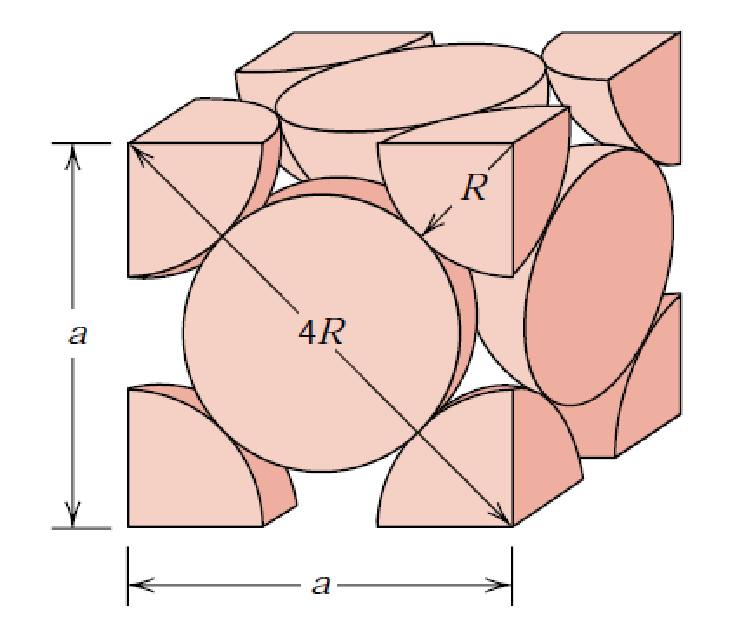
\includegraphics[width=.5\linewidth]{CFC calcolo}
                \end{figure}
                \begin{gather}
                    (4R)^2 = a^2 + a^2 \\
                    a = \frac{4}{\sqrt{2}} R \label{CFC_reference}\\
                    a^3 \cong 22,63 R^3
                \end{gather}
                Il fatto che la lunghezza dei lati $a$ nel reticolo CCC (\ref{CCC_reference}) e' piu' piccolo di $a$ nel reticolo CFC 
                (\ref{CFC_reference}) spiega matematicamente perche' il reticolo CFC e' piu' voluminoso del retiolo CCC.
            \subsubsection{Fattori di compattizione atomica (APF) per il reticolo CFC}
                \begin{gather}
                    V_\text{atomi} = 4 * \frac{4}{3} \pi  R^3 \cong 16,76 R^3 \\
                    V_\text{cella} \cong 22,63 \\
                    APF_\text{CFC} = \frac{V_\text{atomi}}{V_\text{cella}} = \frac{16,76 R^3}{22,63 R^3} \cong 0,74
                \end{gather}
                $\Longrightarrow$ Il volume del reticolo CFC e' occupato il 68\% da atomi.

            \subsection{Regione per il cambio di deformabilita'}
                La deformabilita' e' causata dalla quantita' di spazio che e' vuota (spazio vuoto si chiama anche lacuna).
                Il reticolo CFC e' piu' deformabile del reticolo CCC perche' anche se ha piu' spazio occupato occupato da atomi (74\%) in confronto al reticolo CCC (68\%), 
                il reticolo CFC e' piu' voluminoso quindi la percentuale piu' piccola di lacune nel reticolo CFC e' piu' grande della percentuale piu' grande del reticolo piu' piccolo.
                Le leghe sono create mettendo atomi di altri elementi nelle lacune. I metalli con il reticolo CFC formano leghe piu' prevalentamente per questa ragione.
        \subsection{Fasi strutturali del ferro}
            \begin{figure}[h!]
                \centering
                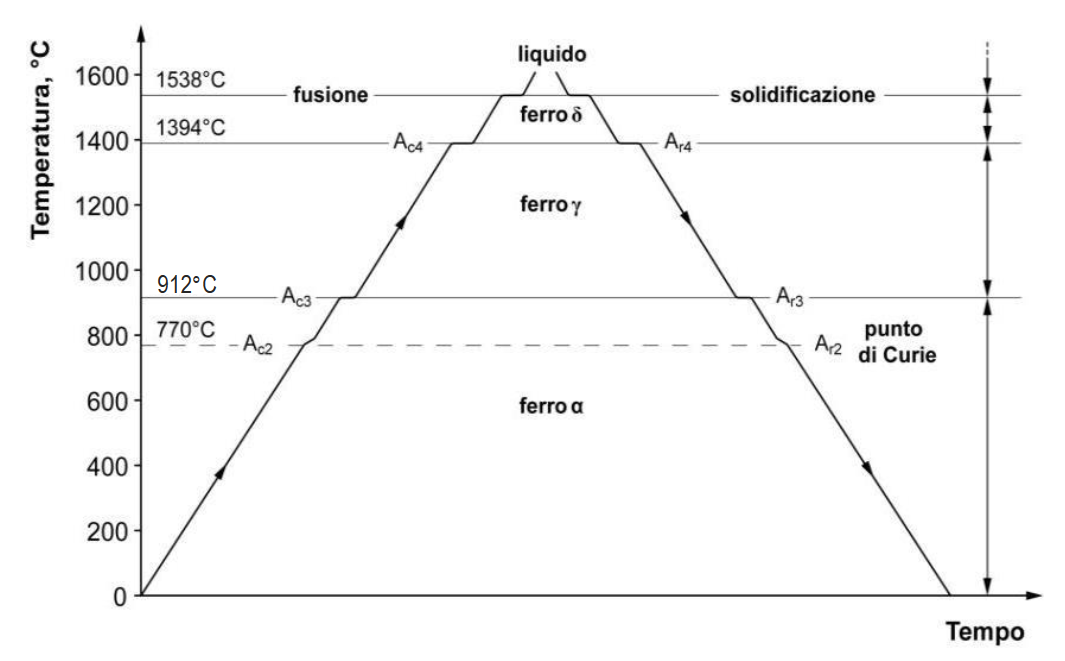
\includegraphics[width=.85\linewidth]{Fasi Ferro.png}
                \end{figure}
            Come cennato prima, il ferro e' un materiale allotropico che significa che cambia forma retticolare al cambio della temperatura.
            Il ferro ha tre fasi retticolari note come $\alpha$ , $\gamma$ e $\delta$. $\alpha$ e $\delta$ sono fasi dove il ferro ha una reticolo CCC 
            invece la nella fase $\gamma$ il ferro ha un reticolo CFC. $\alpha$ e $\delta$ sono chiamati diversamente per facilitare la identificazione 
            della temperatura.
            \newline \newline Gli scalini (punti critici, notati da A\textsubscript{cn} e A\textsubscript{rn}), occorrono quando c'e' un cambio nel 
            ferro in cui c'e' bisogno di energia per effettuarlo.
            \newline \newline Un punto critico nella struttura (A\textsubscript{c2} e A\textsubscript{r2}) e' il "Punto di Curie", questo non 
            occorre quando la struttura del ferro cambia invece a questa temperatura il ferro perde il suo ferromagnetismo e diventa amagnetico.
            \begin{figure}[h!]
                \centering
                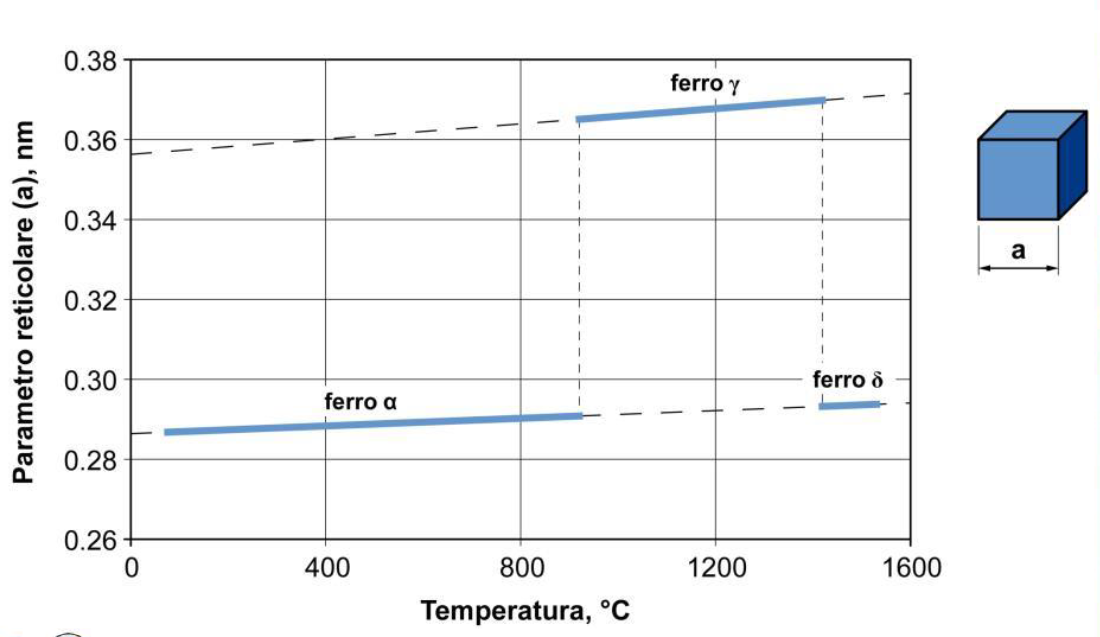
\includegraphics[width=.85\linewidth]{Cambio parametro reticolare nel ferro.png}
            \end{figure} 
            Questa figure mette in evidenza il cambio del parametro reticolare, cioe' la lunghezza di un lato di una celle elementare, nel ferro 
            con il cambio della temperatura e con se il cambio della struttura reticolare.
    \newpage
    \section{Lezione 3 - Reticoli, e diffetti e i loro positivi}    
        \subsection{Reticolo esagonale compatto (HCP)}
            \begin{figure}[ht!]
                \centering
                \begin{subfigure}{.25\linewidth}
                    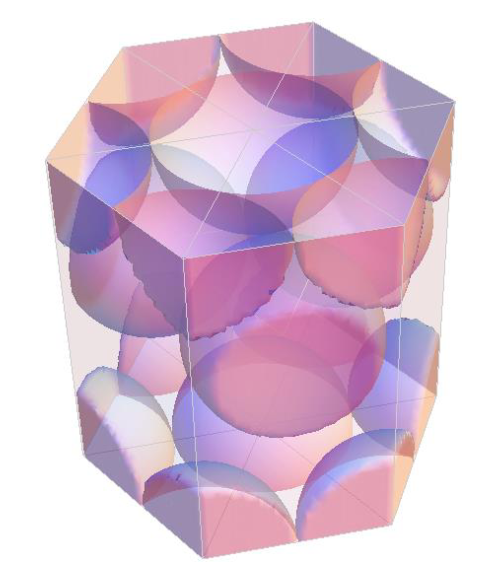
\includegraphics[width=\linewidth]{HCP grafico.png}
                \end{subfigure}
                \begin{subfigure}{.65\linewidth}
                    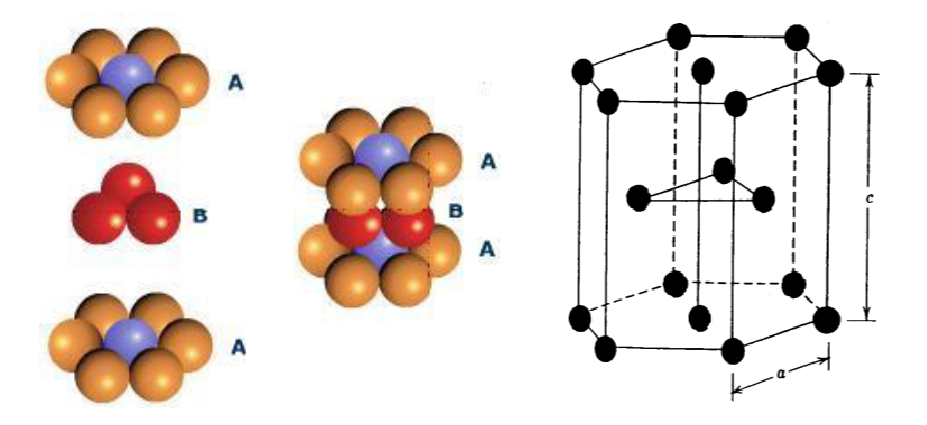
\includegraphics[width=\linewidth]{HCP schematica.png}
                \end{subfigure}
            \end{figure}
            Il reticolo esagonale compatto (HCP) e' usato dal titanio quando $T<882^o C$, dal magnesio, lo zinco, il cadmio e il cobalto. 
            Questi metalli sono resistenti ma \textcolor{red}{fragili} (fragile = tendenza a rompersi come il vetro). Aggiunto al costo piu' basso, l'accaio e' meglio del titanio 
            perche' a piu' \textcolor{red}{tenace} (tenace opposto di fragile).
            \newline \newline Il HCP ha un APF $=0,74$ ed e' composto da 6 atomi propri.

        \subsection{Difetti dei reticoli}
        Ogni reticolo contiene difetti perche' niente e' perfetto, i difetti nei reticolo sono (per la maggior parte) positivi e aiutano con delle 
        proprita dei metalli.
            \subsubsection{Difetti di punto}
                \paragraph{Vacanza} \mbox{}\\
                Una vacanza e' quando c'e' una mancanza di atomi in un certo punto, che cause la compressione degli atomi circostanti a causa di forze repulsiv piu' 
                deboli di se ci fosse un altro atomo.
                \paragraph{Atomi sostituzionali} \mbox{} \\
                Un atomo sostituzionale e' un atomo di una altro elemento che sostituisce un atomo del elemento principale. Questo e' uno dei due metodi per createre 
                le leghe, quindi tecnicamente le leghe sono metalli con difetti.
                \newline \newline Un esempio di una lega creata da atomi sostituzionali e' l'otone che creato da 60\% rame e 40\% zinco.
                \begin{figure}[ht]
                    \centering
                    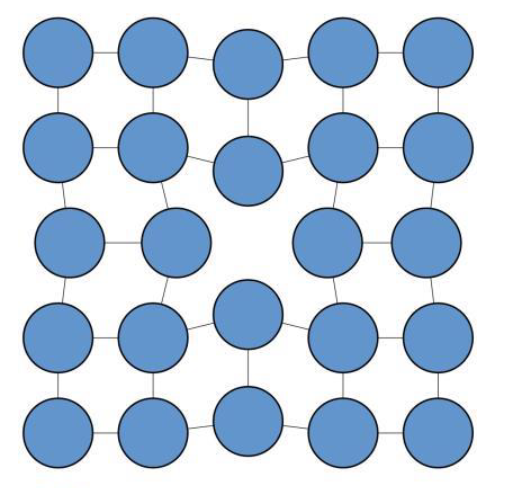
\includegraphics[width=.5\linewidth]{Vacanze.png}
                    \caption{Diagramma semplice di una vacanza reticolare.}
                \end{figure}
                \begin{figure}[ht]
                    \centering
                    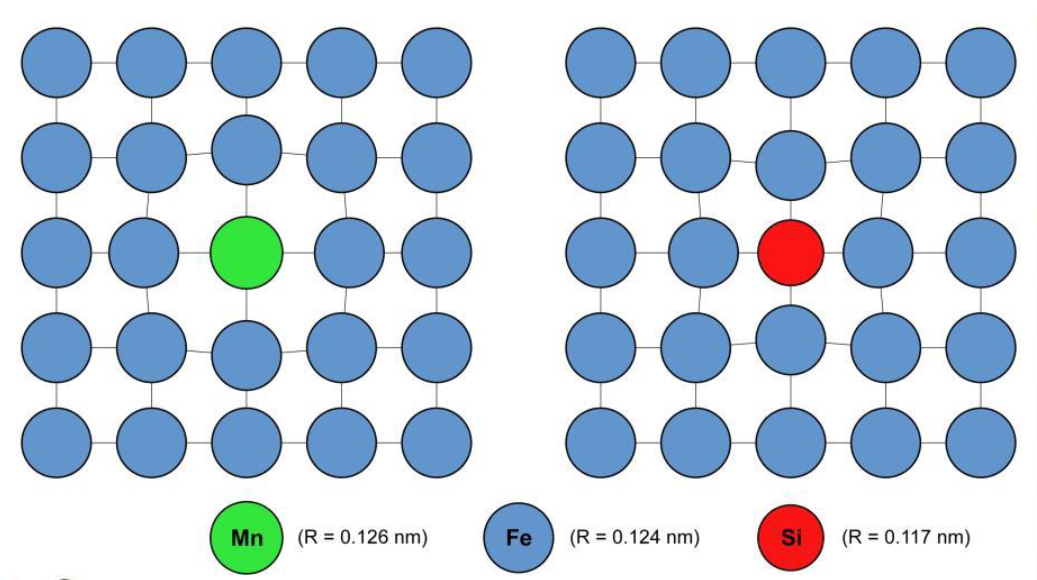
\includegraphics[width=.85\linewidth]{Sostituzione.png}
                \end{figure}
                \newline \newline Nella sostituzione gli atomi che sostituiscono devono essere di dimensioni simili all'atomo principale, se sono troppo grandi i due elementi non sono solubili, 
                e quindi non si crea una lega. Se gli atomi sono di dimensione simile la struttura cambia in corrispondenza alla dimensione dell'atomo sostituente. Se l'atomo e' piu' grande 
                dell'atomo principale, il reticolo circostante si espande a cause di forze repulsive piu' forti, mentre se il diametro e' piu' piccole dell'atomo originale, il reticolo 
                ciscostante si restringe a cause di forze repulsive piu' deboli.
                \paragraph{Atomi interstiziali}\mbox \\
                Un atomo interstiziale e' un atomo decisamente piu' piccolo degli atomi dell'elemento originale che si mette nei buchi del reticolo e cause distrubi alle struttura. Questi 
                disturbi sono piu' grandi dei disturbi che sono creati dagli atomi sostituzionali, qui gli atomi interseziali hanno un effetto piu' grande sulla resistenza di un reticoli 
                che gli atomi sostituzionali.
                \begin{figure}[ht]
                    \centering
                    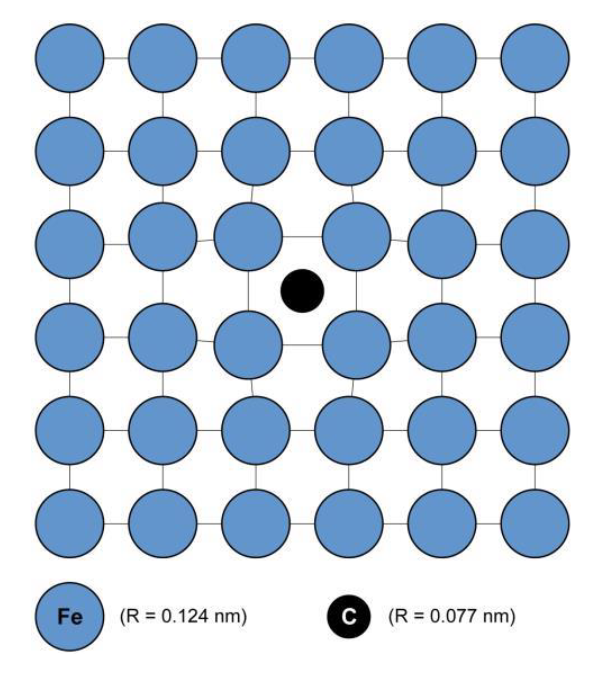
\includegraphics[width=.85\linewidth]{Interstiziali.png}
                \end{figure}
                Un combinazione di atomi sostituzionali e interstiziali e' la cosa migliore per creare un reticolo resistente.
        \subsection{Leghe vs. Metalli Puri}
            Le leghe sono piu' resistenti alle deformazioni a cause dei loro difetti, i difetti causano disturbi al reticolo che lo rendono piu' resistenti alle deformazione.
            Questo disturbi occorro nella forma di una perturbazione del campo elettromagnetico nel retticolo e per cio' la resistenza aumenta.
            \begin{figure}[ht]
                \centering
                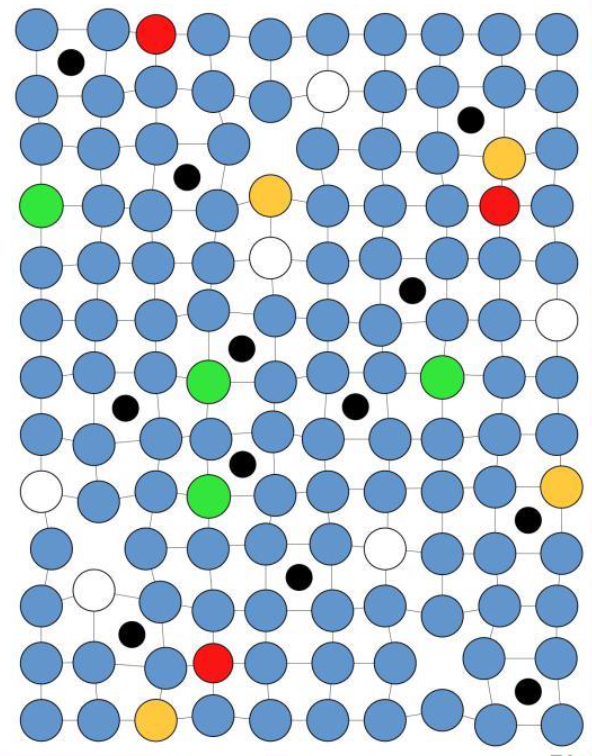
\includegraphics[width=.75\linewidth]{Reticolo Accaio.png}
            \end{figure}
            Nella figure si vede un diagramma del reticolo d'accaio (non esatto), questo rappresenta il fatto che l'accaio e' una lega base ferro e carbonio, ma contiene anche molti 
            altri elementi che cambiano se stessi la struttura.
        \subsection{Rafforzamento per soluzione solida/rafforzamento per alligazione (creano una lega)}
            \begin{figure}[ht]
                \centering
                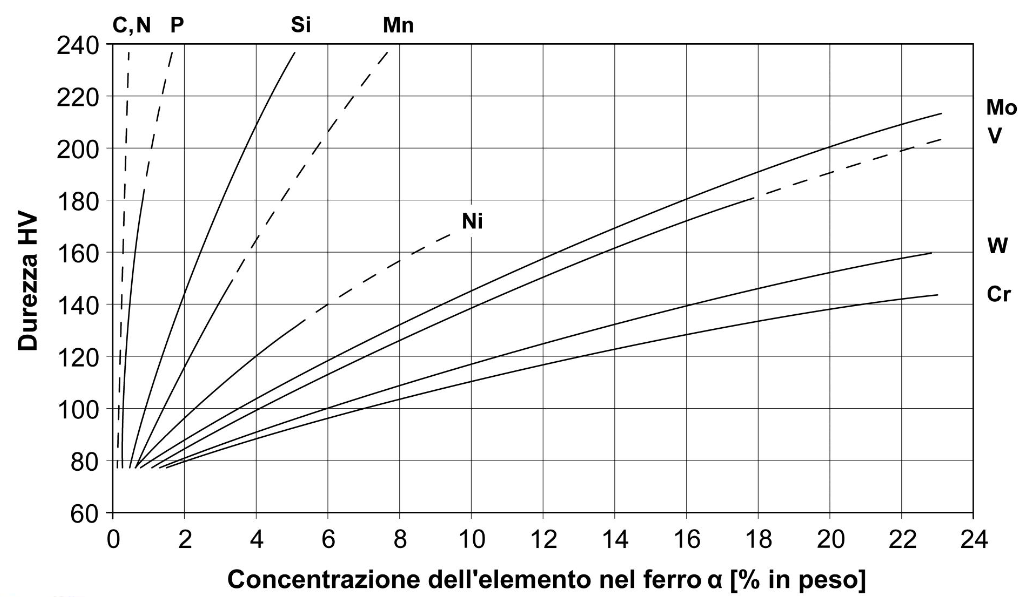
\includegraphics[width=.85\linewidth]{Rafforzamento per soluzione solida.png}
            \end{figure}
            Il diagramma rappresenta la quantita di certi elementi che devono essere aggiunti al ferro per aumentare la durezza di una certa quantita'.
            Quello che possiamo vedere e' che il carbonio e azoto, che sono atomi interstiziali per il ferro aumentano la durezza con una concentrazione 
            molto bassa invece altri metalli che sono atomi sostituzionali per il ferro hanno un effetto piu' basso con concentrazioni piu' elevate, questo 
            di nuovo rafforza l'idea che gli atomi interstiziali hanno un effetto grande sulla resistenza delle leghe.
        \subsection{Reticolo cristallino disordinato/ordinato}
            I reticoli disordinati sono piu' resistenti dei reticoli ordinati.
            \begin{figure}[ht]
                \centering
                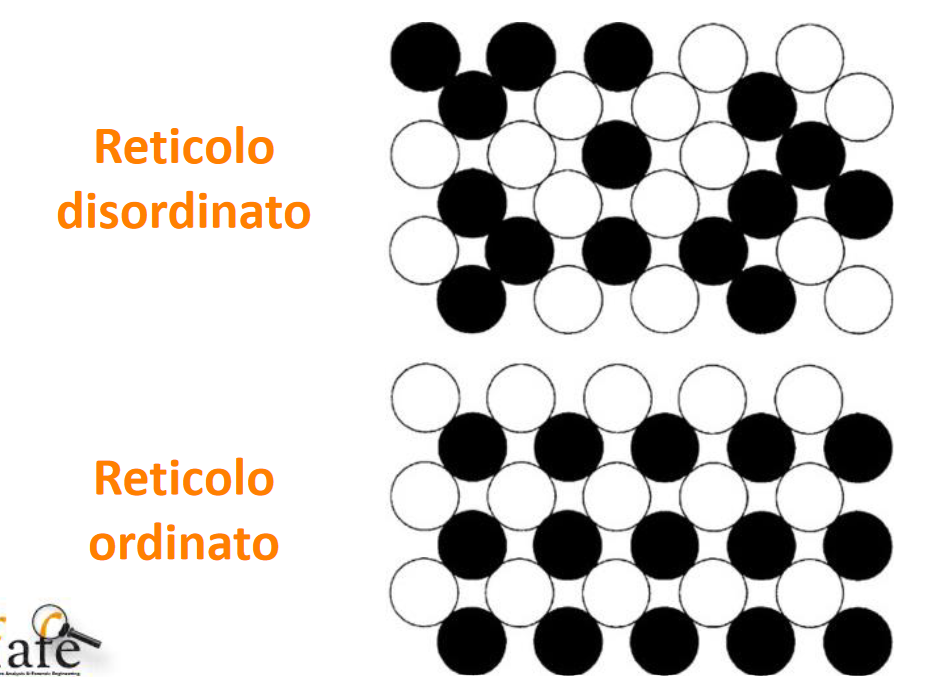
\includegraphics[width=.75\linewidth]{Disordinato Ordinato.png}
            \end{figure}
        \subsection{Solubilita' tra elementi e composti}
        Gli elementi hanno diverse compabilita' con l'un l'altro, alcuni elementi si mischiano bene ad ogni temperatura. Alcuni elementi non si mischiano 
        molto e estiste un limite alla loro solubilita' e se il limite e' passato non si mischiano piu', mentre alcuni elementi non si mischiano a qualsiasi temperature.
        Questo effetto si piu' spiegare con gli atomi sostituzionali e interstiziali. Come detto prima negli atomi atomi sostituzionali, se gli atomi hanno dimensioni 
        troppo diverse non si mischiano, invence con gli atomi interstiziali si crea il limite perche' causano troppi disturbo al reticolo del materiale e quindi troppo 
        causerebbe una deformazione del reticolo.
        \begin{figure}
            \centering
            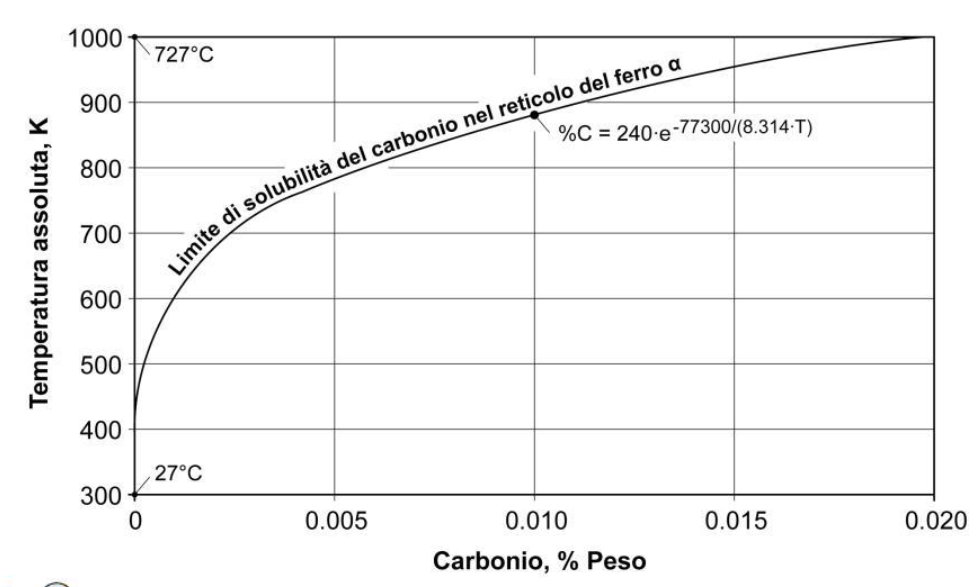
\includegraphics[width=.85\linewidth]{Solubilita'.png}
            \caption{Questo grafico rappresenta la linea del limite di solubilita' tra il carbonio e il ferro e spiega perche ci si mette cosi poco carbonio nell'accaio.}
        \end{figure}
        \newline \newline Ci sono 4 classi di rapporti nella solubilita' di elementi, gli elementi possono:
        \begin{itemize}
            \item Avere perfetta solubilita' (Ag e Au)
            \item Avere parziale solubilta' (Fe e C)(Limite)
            \item Avere perfetta insolubilta' (Fe Pb)
        \end{itemize}
        \subsubsection{Composti Chimici}
            La quarta possibilita' di solubilita' tra 2 elementi e' che creino un composto chimico invece di mischiarsi.
            Per esempi il Fe o O, che quando mischiati creano FeO, un composto ionico.
            I composti possono non avere niente a che fare con il composto e sono completamente inglobati dal reticolo. 
            Le dimensioni interatomiche nel composto sono di solito simili a quelle del reticolo che lo inglobano.
            \newline \newline I composti vengono in due tipi, i composti coerenti e i composti incoerenti.
            \begin{figure}
                \centering
                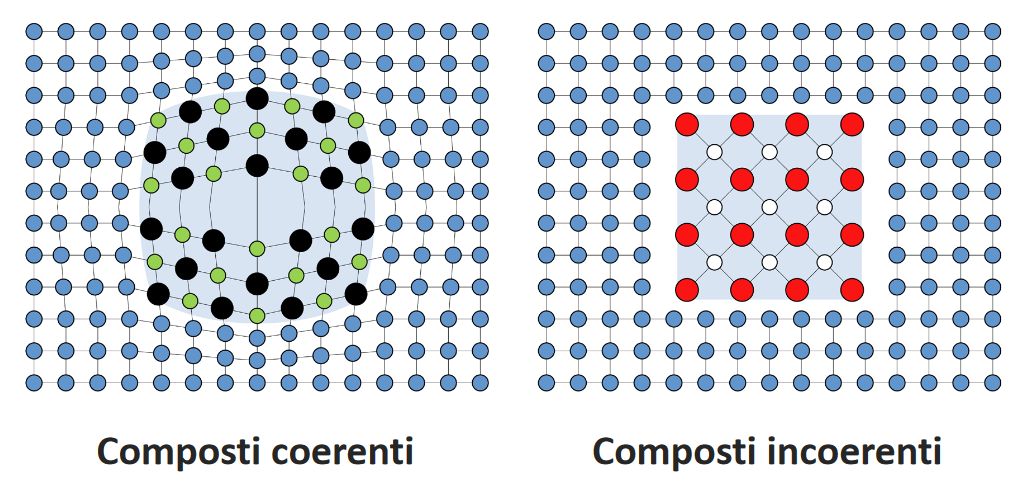
\includegraphics[width=.85\linewidth]{Tipi di Composti.png}
            \end{figure}
            La coerenza ha a che fare con l'orientamento del composto in confronto al reticolo. I composti coerenti, hanno un orientamento che e' uguale a quella del 
            reticolo inglobante e questo permette al composto di creare legami con il reticolo, invece in composti incoerenti il composto un orientamento diverso dal 
            reticolo inglobante per cio' il composto non puo' creare legami con il reticolo inglobante.



                

                
                

\end{document}